\begin{frame}
	\frametitle{Characteristics of Boron\footfullcite{RN3}}
	\begin{minipage}{\linewidth}
		
	
	\begin{minipage}[t]{0.45\linewidth}
		\begin{table}
		\caption{Atomic Radii}
		\begin{tabular}{ccc}
			\toprule
			&B&C\\
			\midrule
			$r_{vdw}$(\AA)&&1.70\\
			$r_{cov}$(\AA)&0.83&0.68\\
			\bottomrule
		\end{tabular}
	\end{table}	
	\end{minipage}
\hspace{0.05\linewidth}
\begin{minipage}[t]{0.45\linewidth}
	\begin{table}
		\caption{Bond Dissociation Energy}
		\begin{tabular}{cl}
			\toprule
			Bonds&$D_{298K}^{^\circ} \ (kJ \cdot mol^{-1})$\\
			\midrule
			\chemfig{B-[,0.5]B}&290\\
			\chemfig{B-[,0.5]H}&$345.2\pm 2.5$\\
			\chemfig{C-[,0.5]C}&$618\pm 15.4$\\
			\chemfig{C-[,0.5]H}&$318.4\pm 1.2$\\
					\chemfig{B-[,0.5]C}&$448\pm 29$\\
			\bottomrule
		\end{tabular}
	\end{table}
\end{minipage}
\end{minipage}
\end{frame}

\begin{frame}
\frametitle{Asymmetric Reduction of \chemfig{C=[,0.6]C}\footfullcite{RN7} and \chemfig{C=[,0.6]O}\footfullcite{RN6} Bonds}
%\setchemfig{fixed length=true}
%\schemestart[0,1.4] \chemname{\chemfig{IPC_2BH}}{99.1\% ee}\arrow{->[\chemfig{-[:30,0.4]=[:330,0.4]-[:30,0.4]}][248 K / 4.5 h]}{\chemfig{{IPC_2B}>[:30,0.6](-[2,0.6]-[:30,0.6])(-[:330,0.6])}}\arrow{->[[O]]}\chemname{\chemfig{{IPC_2B}>[:30,0.6](-[2,0.6]-[:30,0.6])(-[:330,0.6])}}{98.1\% ee} \schemestop
\begin{figure}
	\centering
	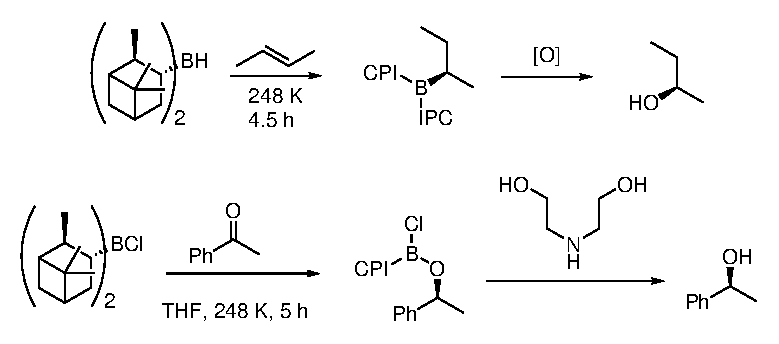
\includegraphics[width=0.9\linewidth]{fig/AsymmetricReduction}
	%\caption{Asymmetric Reduction of \chemfig{C=[,0.6]C} and \chemfig{C=[,0.6]O}}
	\label{fig:asymmetricreduction}
\end{figure}

\end{frame}

\begin{frame}
\frametitle{Diastereoselective Allylboration\footfullcite{RN4}}
\begin{figure}
	\centering
	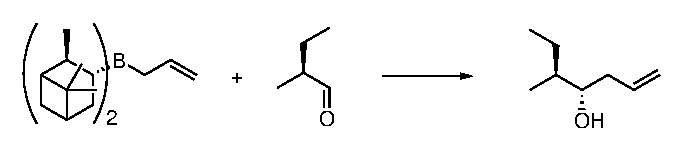
\includegraphics[width=0.8\linewidth]{fig/diastereo}
	\caption{Diastereoselective Allylboration}
	\label{fig:diastereo}
\end{figure}

\end{frame}

\begin{frame}
	\frametitle{Suzuki-Miyaura Cross-Coupling}
	\begin{figure}
		\centering
		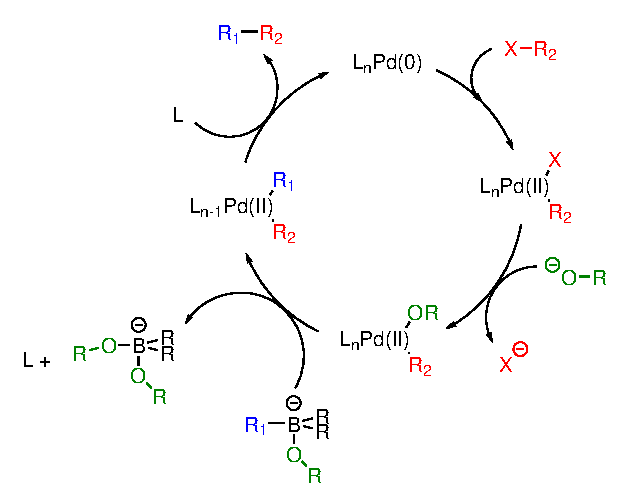
\includegraphics[width=0.7\linewidth]{fig/suzuki-miyaura}
		%\caption{}
		\label{fig:suzuki-miyaura}
	\end{figure}
	
\end{frame}